	\section{Resultados Y Análisis}
		\subsection{Caracterización eléctrica del reactor}
En la Fig. \ref{fig:Señales Típicas} se muestran señales típicas de corriente (en verde) y voltaje (en rojo) al alimentar al sistema con $V_{\tx{AC}} = (15,0 \pm 0,2) \n{kV}$ pico a pico de tensión alterna. Se observa que la corriente presenta picos correspondientes a la corriente de streamers $I_{\tx{str}}$ medida a la salida del E3. \\
\begin{figure}[!htbp] \centering
    \vspace{-.4cm}
    \SB{1}{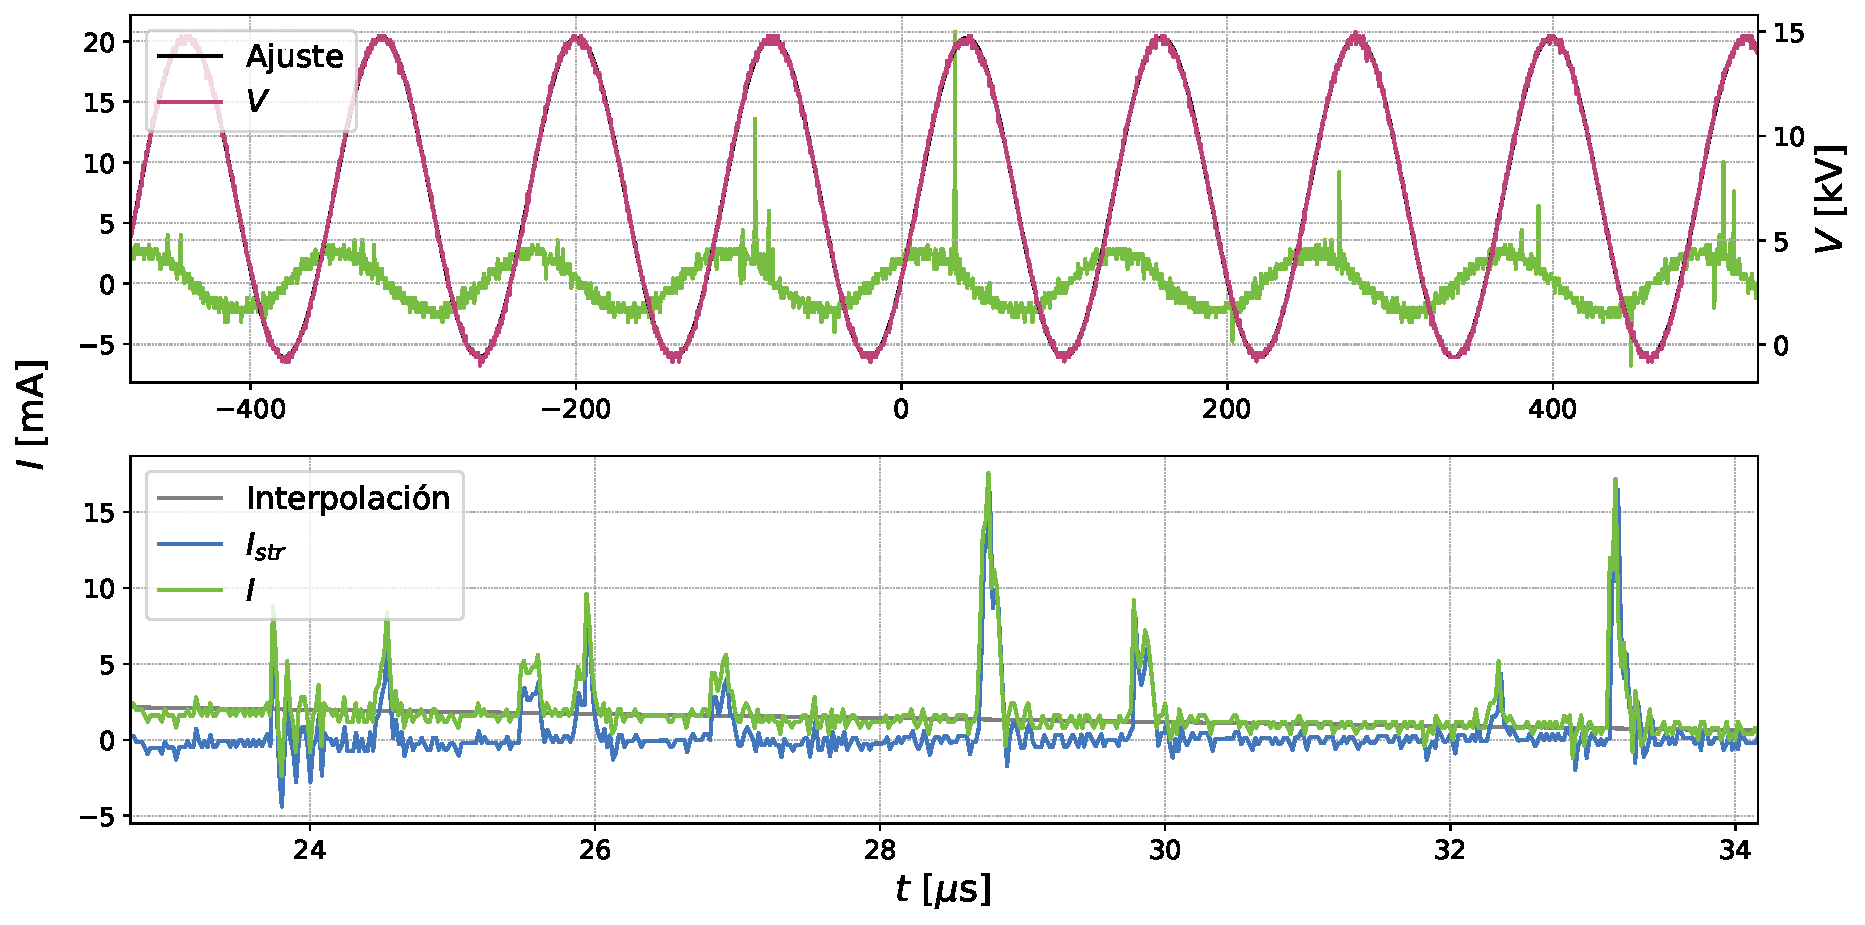
\includegraphics[width=0.85\textwidth]{Figuras/Señales_Típicas.pdf}}
    \vspace{-.3cm}
    \caption{señales típicas de la corriente (en verde) y el voltaje (en rojo) con su ajuste sinusoidal (en negro). En la figura inferior se observa una medición ampliada de la corriente con su interpolación (en gris) y la corriente de streamers $I_{\tx{str}}$ obtenida (en azul).}
    \label{fig:Señales Típicas}
\end{figure}

La potencia eléctrica es un parámetro importante del sistema ya que da una idea de la eficiencia energética del tratamiento. Para calcularla, se define a la potencia media como:
\begin{equation*}
    \langle P \rangle = \frac{1}{T} \int_0^T I_{\tx{str}} V \,\text{d}t,
\end{equation*}
donde $T$ es el período, $I_{\tx{str}}$ la corriente de streamers y $V = V_{\tx{AC}} + V_{\tx{DC}}$ es la diferencia de potencial entre los electrodos E1 y E3. Para obtener el período, es necesario tomar una medición donde se aprecie el comportamiento sinusoidal del voltaje y así poder realizarle un ajuste. Luego se aumenta la resolución temporal para definir más precisamente a los picos de corriente, que se detectan cuando los streamers cruzan del sistema E1-E2 al E3. Sin embargo, sobre esta señal ampliada todavía hay que suprimir la componente senoidal, que da cuenta de las corrientes capacitivas y no de la corriente de streamers. Para ello, se toman como referencia al primer y último pico de la corriente y se interpola una recta entre estos dos puntos. Luego se resta esta señal de base a la señal de corriente y de ahí se obtiene $I_{\tx{str}}$, como se muestra en la Fig. \ref{fig:Señales Típicas} (en azul). \\\\
Con este procedimiento, utilizando una tensión continua de $10 \n{kV}$ se calculó la potencia promedio para los sistemas de electrodos de acrílico, teflón y vidrio, descriptos en la sección anterior. Dichos resultados pueden observarse en la Fig. \ref{fig:Potencias}, donde se grafica la potencia en función del voltaje pico a pico. Las mediciones se tomaron dentro del rango de funcionamiento de los sistemas de electrodos (es decir, donde no producían chispas). Cabe notar que el vidrio fue el material dieléctrico con mayor rango de funcionamiento, siendo que el teflón y el acrílico no siempre generaban una DBD uniforme. Esto se debe a que la superficie del vidrio es más uniforme que la de los otros materiales, lo cual evita la generación de canales preferenciados por donde se formen streamers. Por otro lado, puede observarse en la Fig. \ref{fig:Potencias} que el sistema de electrodos de teflón requería menos tensión que el de vidrio para alcanzar la misma potencia, necesitando el acrílico un valor de tensión intermedio entre ambos. Esto tiene sentido si se tiene en cuenta que la constante dieléctrica del teflón es menor a la del vidrio \cita{15}, con lo cual más voltaje es necesario para generar la DBD.

\begin{figure}[!htbp] \centering
    \vspace{-.5cm}
    \SB{1}{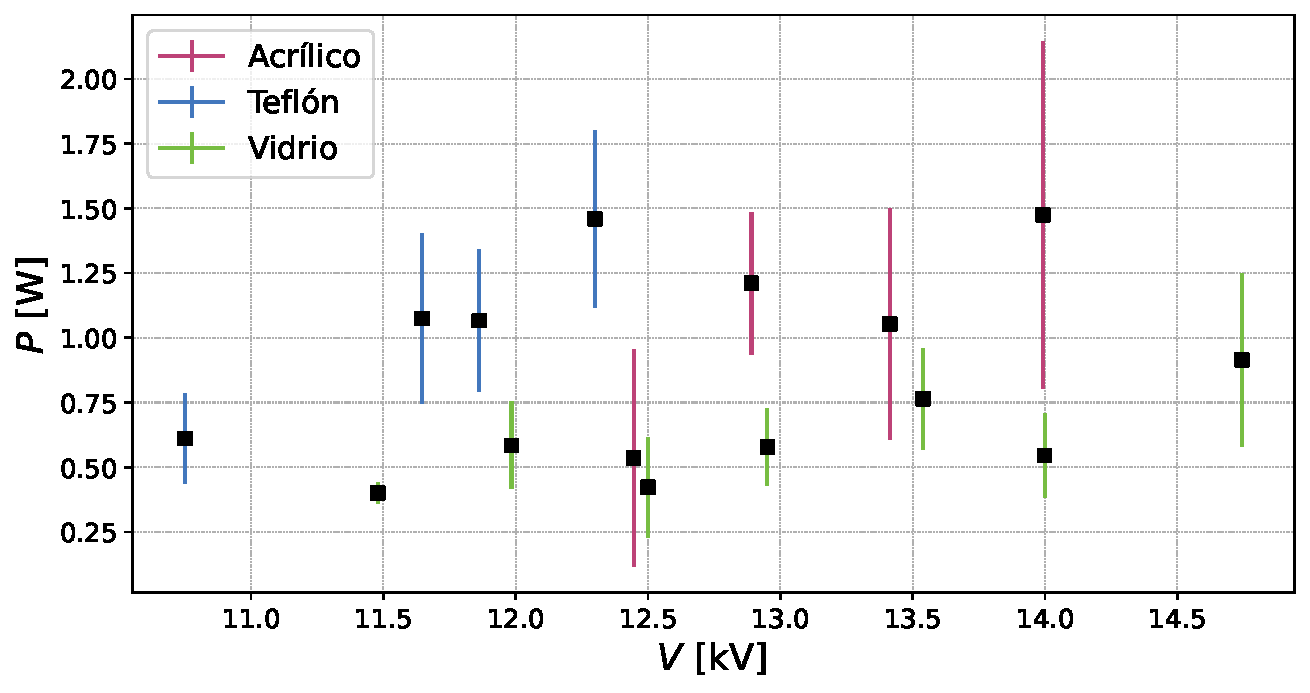
\includegraphics[width=0.75\textwidth]{Figuras/Potencias.pdf}}
    \vspace{-.4cm}
    \caption{potencia promedio para distintos materiales dieléctricos a diferentes tensiones.}
    \label{fig:Potencias}
\end{figure}
		\subsection{Estudio del azul de metileno}
Con el fin de evaluar la eficiencia en la remoción de contaminantes del reactor, se utilizaron soluciones de \txcurs{azul de metileno} ($\tx{C}_{16}\tx{H}_{18}\tx{ClN}_3\tx{S}$) diluido en agua Milli-Q como prototipo de agua contaminada \cita{9}. Con un espectrofotómetro BioTraza Modelo 721 se midió el espectro de absorción del azul de metileno para una concentración de $10 \n{ppm}$, como se observa en la Fig. \ref{Absorbancia}. Para obtener dicha solución, se pesaron $(10,0 \pm 0,2) \n{mg}$ de azul con una balanza y se los diluyeron en $(1 \pm 0,002) \n{L}$ de agua Milli-Q. Se graficó la absorbancia con respecto a la longitud de onda y se encontró al máximo absoluto del espectro en $\lamda_{\tx{máx}} = (662 \pm 1) \n{nm}$, lo cual coincide con el valor tabulado \cita{16}. \\
\vspace{-.25cm}
\begin{figure}[!htbp] \centering
    \vspace{-.5cm}
	\subfloat[][]{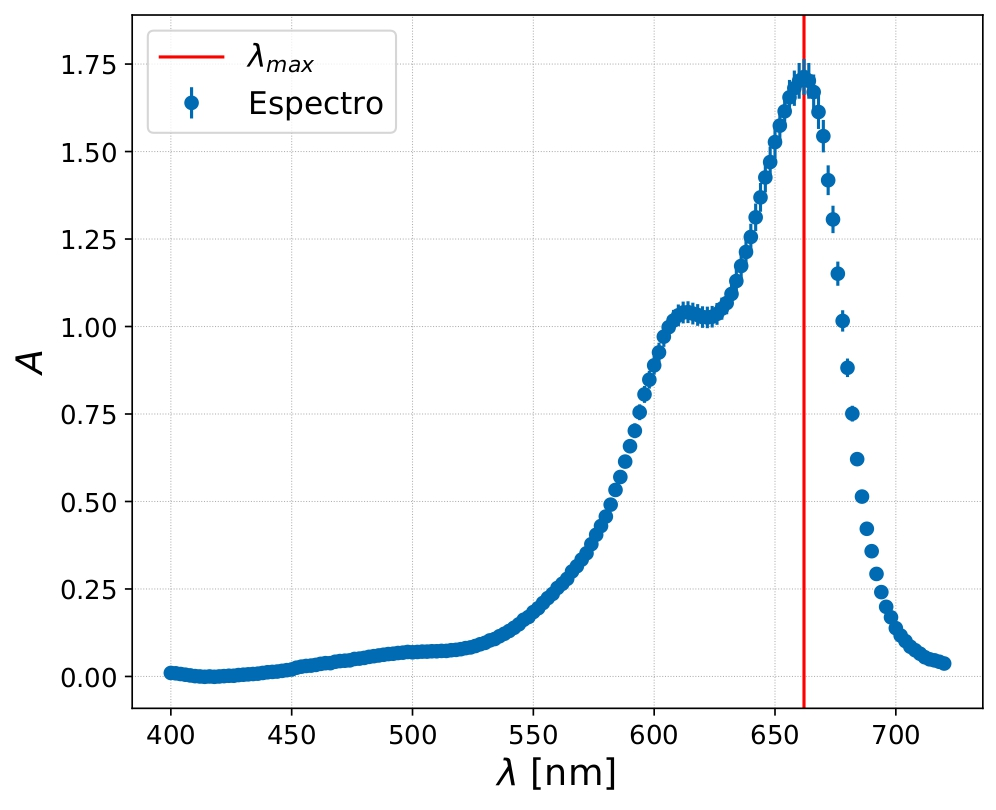
\includegraphics[scale=0.55]{Figuras/Absorbancia.png}\label{Absorbancia}}
	\subfloat[][]{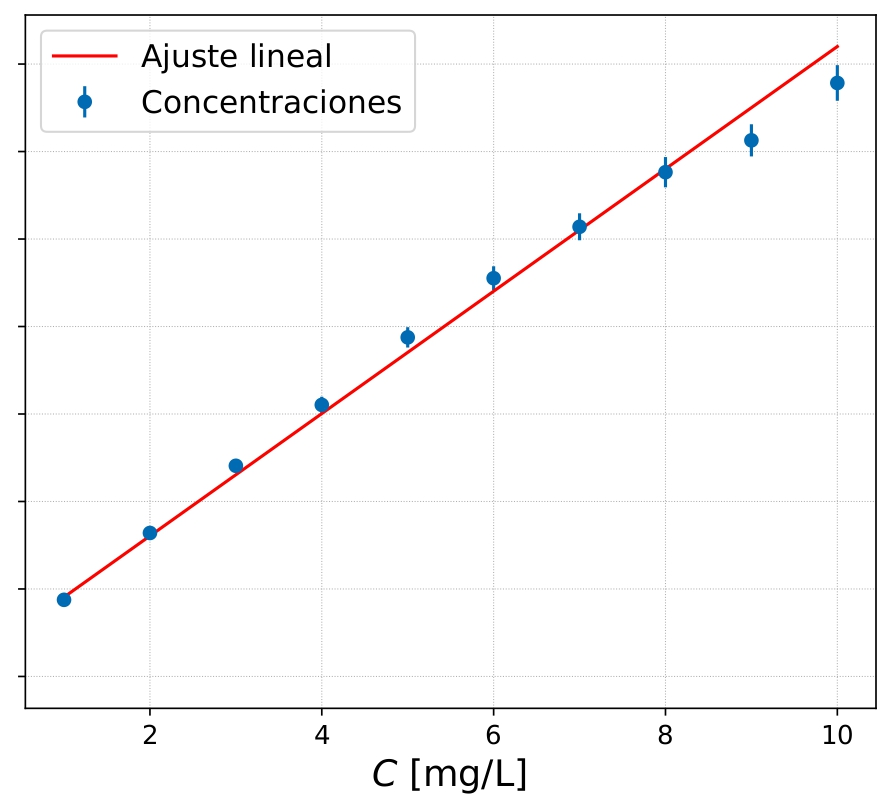
\includegraphics[scale=0.55]{Figuras/Ajuste Lineal.png}\label{Ajuste Lineal}}
	\vspace{-.25cm}
	\caption{\protect\subref{Absorbancia} espectro de absorbancia. \protect\subref{Ajuste Lineal} ajuste lineal de la absorbancia con respecto a la concentración.}
\end{figure}

Con el fin de verificar la ley de Lambert-Beer, que indica la proporcionalidad directa entre la concentración y la absorbancia de una muestra \cita{14}, se fueron diluyendo $10 \n{ppm}$ de azul de metileno en agua Milli-Q y se midió la absorbancia para las diferentes concentraciones. Para esto, a la concentración inicial se le fueron agregando ente $10$ y $500 \n{ml}$ de agua Milli-Q, medidas en una probeta con una incerteza de $1 \n{ml}$. En la Fig. \ref{Ajuste Lineal} se puede observar la linealidad entre la concentración y la absorbancia en el rango de trabajo para el tratamiento. De esta forma, las mediciones de absorbancia se corresponden con la concentración de la muestra.
		\subsection{Tratamiento de aguas contaminadas}
Para el tratamiento de las soluciones acuosas de azul de metileno se trabajó en las siguientes condiciones: se vertieron en el vaso de precipitado $200 \n{ml}$ de azul de metileno a una concentración de $10 \n{ppm}$ y se trató la solución durante $140 \n{min}$, tomando alícuotas sobre las que se midió absorbancia cada $5 \n{min}$ de tratamiento. Todos los ensayos se realizaron empleando un único sistema de electrodos y alimentando al sistema con $7 \n{kV}$ de tensión continua y $16 \n{kV}$ de tensión alterna. Se realizaron pausas de cinco a diez minutos a los $40, 60$ ó $90$ minutos de tratamiento para evitar el sobrecalentamiento del reactor.  \\\\
Para analizar cuantitativamente los tratamientos y comparar con otros trabajos es útil definir la eficiencia de degradación ($DE$) \cita{9}:
\begin{equation*}
    DE = \fr{C_0-C_t}{C_0} \Por 100 \%,
\end{equation*}
donde $C_0$ y $C_t$ son la concentración al comenzar y al finalizar el tratamiento. Como se observa de su definición, el $DE$ mide el porcentaje de contaminante degradado. Otro parámetro importante es el rendimiento energético ($Y$), que cuantifica cuánto volumen $V$ se degradó en relación a cuánta energía $P \Por t$ se utilizó. Se define como:
\begin{equation*}
    Y = \fr{6 \Por C_0 \Por DE \Por V}{10^4 \Por P \Por t} \, \lb{\fr{\tx{g}}{\tx{kW} \por \tx{h}}}\rb,
\end{equation*}
donde $V$ es el volumen de la solución tratada.
			\subsubsection{Tratamiento con diferentes sistemas de electrodos}
En la Fig. \ref{fig:Degradaciones} se presentan alícuotas de la solución de azul de metileno tomadas durante un tratamiento en el que se empleó un electrodo de teflón sin $\tx{TiO}_2$. Se observa que las muestras se hacen cada vez más transparentes a medida que se degrada el azul de metileno. \\
\begin{figure}[!htbp] \centering
    \vspace{-.5cm}
    \SB{1}{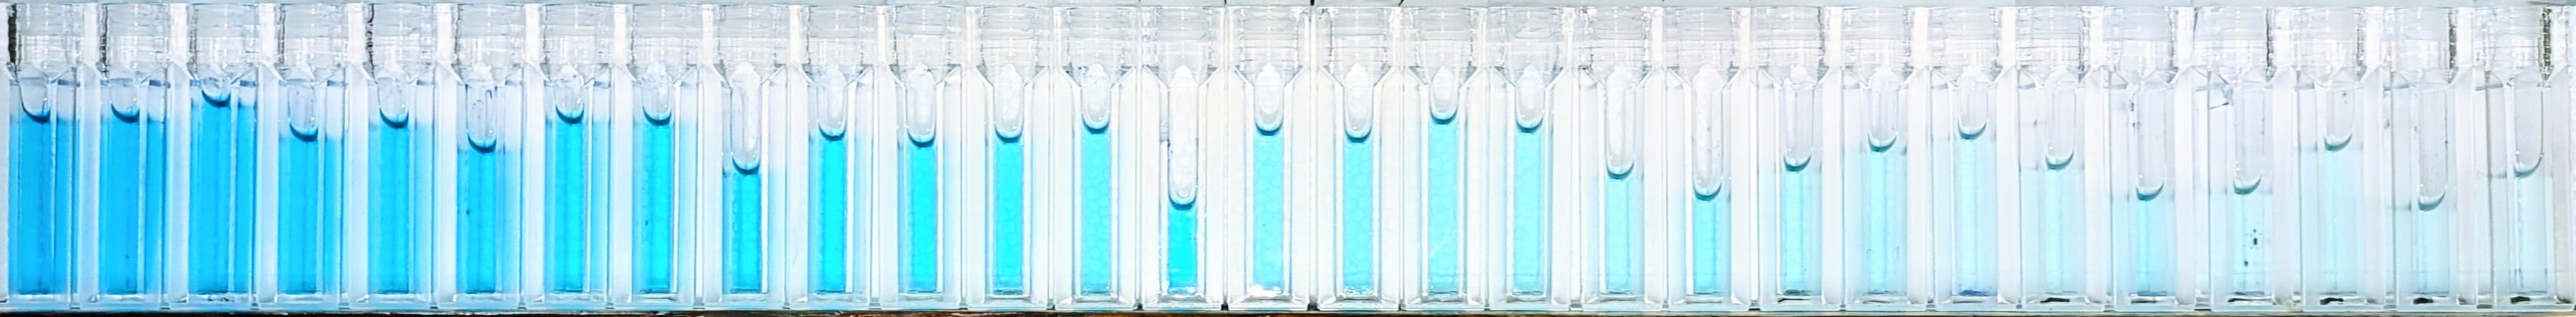
\includegraphics[width=.7\textwidth]{Figuras/Degradaciones.jpg}}
    \caption{alícuotas de las soluciones acuosas de azul de metileno al ser tratadas durante $140$ minutos con el sistema de teflón sin $\tx{TiO}_2$.}
    \label{fig:Degradaciones}
\end{figure}

En la Fig. \ref{fig:Tratamiento_Dielectricos} se muestra esta degradación para distintos sistemas de electrodos E1-E2 de manera cuantitativa. \\
\begin{figure}[!htbp] \centering
    \vspace{-.5cm}
    \SB{1}{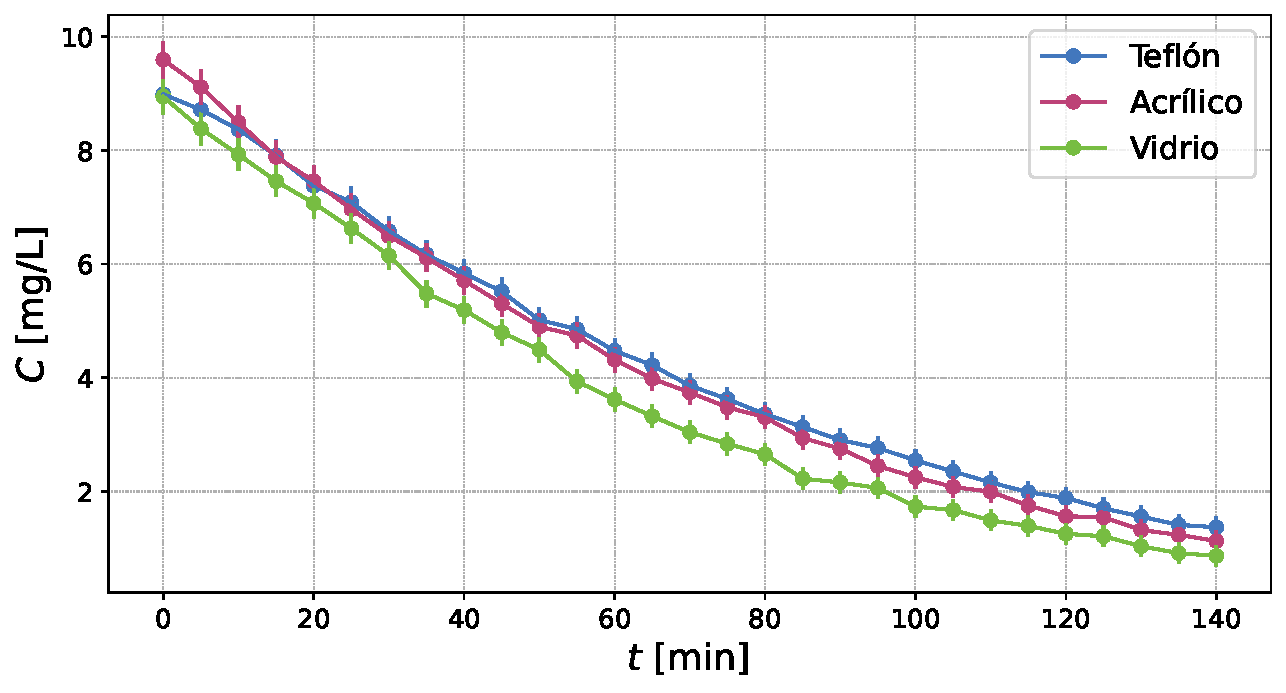
\includegraphics[width=.7\textwidth]{Figuras/Tratamiento_Dielectricos.pdf}}
    \vspace{-.4cm}
    \caption{concentración en función del tiempo empleando distintos materiales dieléctricos.}
    \label{fig:Tratamiento_Dielectricos}
\end{figure}

Como se puede observar, las curvas de concentración se mantienen sin diferencias significativas. Esto se debe a que las tensiones y corrientes fueron iguales dentro del error en los tres tratamientos. La leve separación en las curvas es atribuible a condiciones externas que pueden haber mejorado o empeorado la descarga, pero esta separación no representa una diferencia apreciable en la eficiencia de degradación. \\
\begin{table}[h!] \centering 
\vspace{-.25cm}
\SB{0.9}{\begin{tabular}{|c|c|c|c|} \hline
\Fa \bf \Tb{Configuración} & \Tb{$P$ (W)} & \Tb{$DE$ (\%)} & \Tb{$Y$ (g/kWh)} \\ \hline
\CaTb{Teflón} & $0,7 \pm 0,2$ & $85 \pm 2$ & $1,0 \pm 0,3$ \\ \hline
\CaTb{Acrílico} & $0,7 \pm 0,3$ & $88 \pm 2$ & $1,1 \pm 0,5$ \\ \hline
\CaTb{Vidrio} & $0,7 \pm 0,3$ & $90 \pm 2$ & $1,0 \pm 0,5$ \\ \hline
\end{tabular}}
\caption{potencia, eficiencia de degradación y rendimiento energético para distintos dieléctricos.}
\label{tab:Tratamiento_Dielectricos}
\end{table}

En la tabla \ref{tab:Tratamiento_Dielectricos} se muestran la potencia, la eficiencia de degradación y el rendimiento energético obtenidos para cada tratamiento. En todos se obtuvieron valores cercanos entre sí, siendo la remoción del $90$ \% del contaminante para el caso del vidrio el mejor resultado. Por otro lado, el rendimiento energético se encuentra dentro de valores intermedios en relación a los reportados en otros trabajos \cita{9}.
			\subsubsection{Tratamiento con dióxido de Titanio}
Se realizaron dos mediciones distintas para estudiar el reactor híbrido. Utilizando únicamente el sistema de electrodos de teflón, se colocó en la canaleta una pieza rectangular de vidrio recubierta con dióxido de titanio, como se muestra en el esquema de la Fig. \ref{fig:Esquema Reactor}. Como control, se realizó otro tratamiento con el mismo vidrio pero sin el recubrimiento, ya que el vidrio mismo actúa como dieléctrico y disminuye la potencia de la descarga. En la Fig. \ref{fig:Tratamiento_Titanio}, se grafican los resultados. \\
\begin{figure}[!htbp] \centering
    \vspace{-.5cm}
    \SB{1}{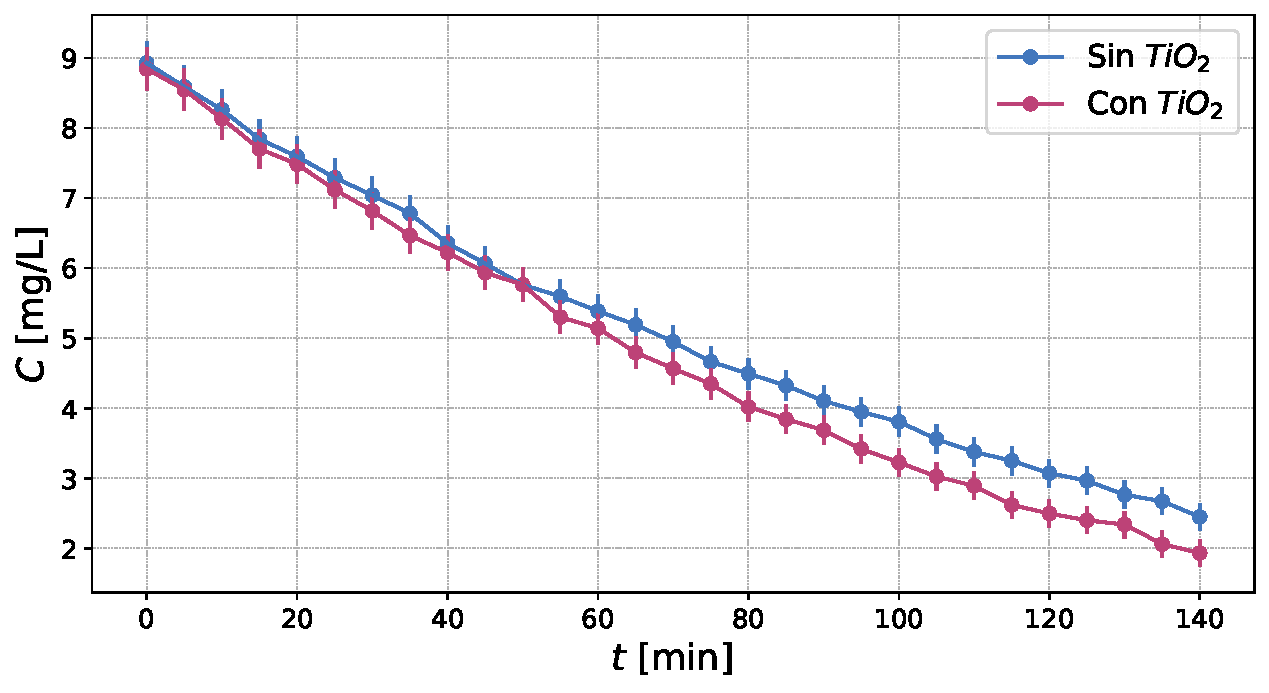
\includegraphics[width=.7\textwidth]{Figuras/Tratamiento_Titanio.pdf}}
    \vspace{-.4cm}
    \caption{concentración en función del tiempo empleando recubrimientos con y sin dióxido de titanio.}
    \label{fig:Tratamiento_Titanio}
\end{figure}

A partir de estas mediciones se observa que con la presencia de titanio se llega a una concentración final ligeramente menor. Esto se confirmó repitiendo la medición y obteniendo resultados similares. Que el impacto del $\tx{TiO}_2$ no haya sido tan notable en el tratamiento, se puede deber a que la radiación ultravioleta emitida por el plasma no sea lo suficentemente intensa como para fotoactivar al material. Para ver más en detalle la diferencia entre los tratamientos con y sin recubrimiento, se presentan en la tabla \ref{tab:Tratamiento_Titanio} las mismas magnitudes que se analizaron antes. \\
\begin{table}[h!] \centering
\vspace{-.25cm}
\SB{0.9}{\begin{tabular}{|c|c|c|c|} \hline
\Fa \bf \Tb{Configuración} & \Tb{$P$ (W)} & \Tb{$DE$ (\%)} & \Tb{$Y$ (g/kWh)} \\ \hline
\CaTb{Sin $\n{TiO}_2$} & $0,5 \pm 0,2$ & $73 \pm 2$ & $1,3 \pm 0,4$ \\ \hline
\CaTb{Con $\n{TiO}_2$} & $0,6 \pm 0,2$ & $78 \pm 2$ & $1,2 \pm 0,5$ \\ \hline
\end{tabular}}
\caption{potencia, eficiencia de degradación y rendimiento energético para el tratamiento con y sin recubrimiento de $\n{TiO}_2$.}
\label{tab:Tratamiento_Titanio}
\end{table}

En la tabla se observa que la presencia de la pieza de vidrio en la canaleta provoca que la potencia del tratamiento sin recubrimiento se reduzca al comparar con el tratamiento con teflón de la tabla \ref{tab:Tratamiento_Dielectricos}. Esto se debe a que el vidrio agregado funciona como material dieléctrico y reduce la corriente y, por lo tanto, la potencia que llega al E3. En consecuencia, la eficiencia de degradación también se reduce. Con esto se concluye que para que el uso del dióxido de titanio sea de utilidad, su efecto deberá superar al dieléctrico agregado o se deberá elegir otro material sobre el que hacer los recubrimientos.